% Options for packages loaded elsewhere
\PassOptionsToPackage{unicode}{hyperref}
\PassOptionsToPackage{hyphens}{url}
%
\documentclass[
]{article}
\usepackage[a4paper, margin=2cm]{geometry}
\usepackage{amsmath,amssymb}
\usepackage{lmodern}
\usepackage{tabularray}
\usepackage{tabularx}
\usepackage{iftex}
\ifPDFTeX
  \usepackage[T1]{fontenc}
  \usepackage[utf8]{inputenc}
  \usepackage{textcomp} % provide euro and other symbols
\else % if luatex or xetex
  \usepackage{unicode-math}
  \defaultfontfeatures{Scale=MatchLowercase}
  \defaultfontfeatures[\rmfamily]{Ligatures=TeX,Scale=1}
\fi
% Use upquote if available, for straight quotes in verbatim environments
\IfFileExists{upquote.sty}{\usepackage{upquote}}{}
\IfFileExists{microtype.sty}{% use microtype if available
  \usepackage[]{microtype}
  \UseMicrotypeSet[protrusion]{basicmath} % disable protrusion for tt fonts
}{}
\makeatletter
\@ifundefined{KOMAClassName}{% if non-KOMA class
  \IfFileExists{parskip.sty}{%
    \usepackage{parskip}
  }{% else
    \setlength{\parindent}{0pt}
    \setlength{\parskip}{6pt plus 2pt minus 1pt}}
}{% if KOMA class
  \KOMAoptions{parskip=half}}
\makeatother
\usepackage{xcolor}
\IfFileExists{xurl.sty}{\usepackage{xurl}}{} % add URL line breaks if available
\IfFileExists{bookmark.sty}{\usepackage{bookmark}}{\usepackage{hyperref}}
\urlstyle{same} % disable monospaced font for URLs
\usepackage{longtable,booktabs,array}
\usepackage{calc} % for calculating minipage widths
% Correct order of tables after \paragraph or \subparagraph
\usepackage{etoolbox}
\makeatletter
\patchcmd\longtable{\par}{\if@noskipsec\mbox{}\fi\par}{}{}
\makeatother
% Allow footnotes in longtable head/foot
\IfFileExists{footnotehyper.sty}{\usepackage{footnotehyper}}{\usepackage{footnote}}
\makesavenoteenv{longtable}
\usepackage{graphicx}
\makeatletter
\def\maxwidth{\ifdim\Gin@nat@width>\linewidth\linewidth\else\Gin@nat@width\fi}
\def\maxheight{\ifdim\Gin@nat@height>\textheight\textheight\else\Gin@nat@height\fi}
\makeatother
% Scale images if necessary, so that they will not overflow the page
% margins by default, and it is still possible to overwrite the defaults
% using explicit options in \includegraphics[width, height, ...]{}
\setkeys{Gin}{width=\maxwidth,height=\maxheight,keepaspectratio}

% Set default figure placement to htbp
\makeatletter
\def\fps@figure{htbp}
\makeatother
\setlength{\emergencystretch}{3em} % prevent overfull lines
\providecommand{\tightlist}{%
  \setlength{\itemsep}{0pt}\setlength{\parskip}{0pt}}
  
% \setcounter{secnumdepth}{-\maxdimen} % remove section numbering

\ifLuaTeX
  \usepackage{selnolig}  % disable illegal ligatures
  \usepackage{rotating}
  \usepackage{amsmath,amssymb} % For mathematical symbols and equations
\usepackage{graphicx} % For including images
\usepackage{float} % To control figure placement
\usepackage{longtable,booktabs,array} % For advanced table formatting
\usepackage{xurl} % Add URL line breaks if available
\usepackage{hyperref} % For hyperlinks
\fi


\title{\LARGE \textbf{Escape Doom - Software Testing Assignment 2}}
\author{Kambal, Nowak, Perov, Selbach, Winter}
\date{\today}

\begin{document}
\maketitle

% --- Table of contents autogenerated ------------------------------------
\newpage
\tableofcontents

\hypertarget{section-introduction-and-goals}{%
\section{Project-Vision and Goals}\label{section:introduction-and-goals}}

The Escape Doom system aims to provide FH Campus Wien with a platform for creating educational escape rooms. In the first semester of our Bachelor’s program, we participated in a programming escape room that offered an engaging, interactive learning experience. Inspired by this positive experience, we want to create a platform that allows students to easily access and play similar escape rooms.


\subsection{Motivation}

Initially, instructors of FH Campus Wien manually created and managed escape rooms by coding each one from scratch. This approach allows for unique, tailored experiences, but it is labor-intensive and difficult to maintain over time, especially as riddles need to be refreshed every one to two years to prevent sharing of solutions between cohorts. This inspired us to develop our own version of an escape room to explore the potential for creating a scalable, reusable platform.

In the current situation, our project—while functional—still requires participants to use an IDE (with the code accessible) which limits usability and makes solutions to code-based challenges more easily discoverable. Our goal is to address these limitations by transforming the project into a streamlined, maintainable system—or in other words, a product—that reinforces the educational value of the escape room.

\subsection{Product Vision}

Our target groups include both students and instructors at FH Campus Wien. For students, we aim to create an escape room platform that enhances learning by providing a fun, interactive environment with near real-time collaboration and an intuitive, browser-based coding experience. For instructors, we aim to provide a maintainable system that allows them to use escape rooms as an educational tool, with the future goal of enabling them to design and configure their own escape rooms.

Our vision is to develop a tool that enables instructors to create and manage user-friendly and accessible point-and-click escape rooms for their courses, with functionality similar to CodinGame escape rooms.\footnote{\url{https://escape.codingame.com/}}



\begin{figure}[h!]
    \centering
    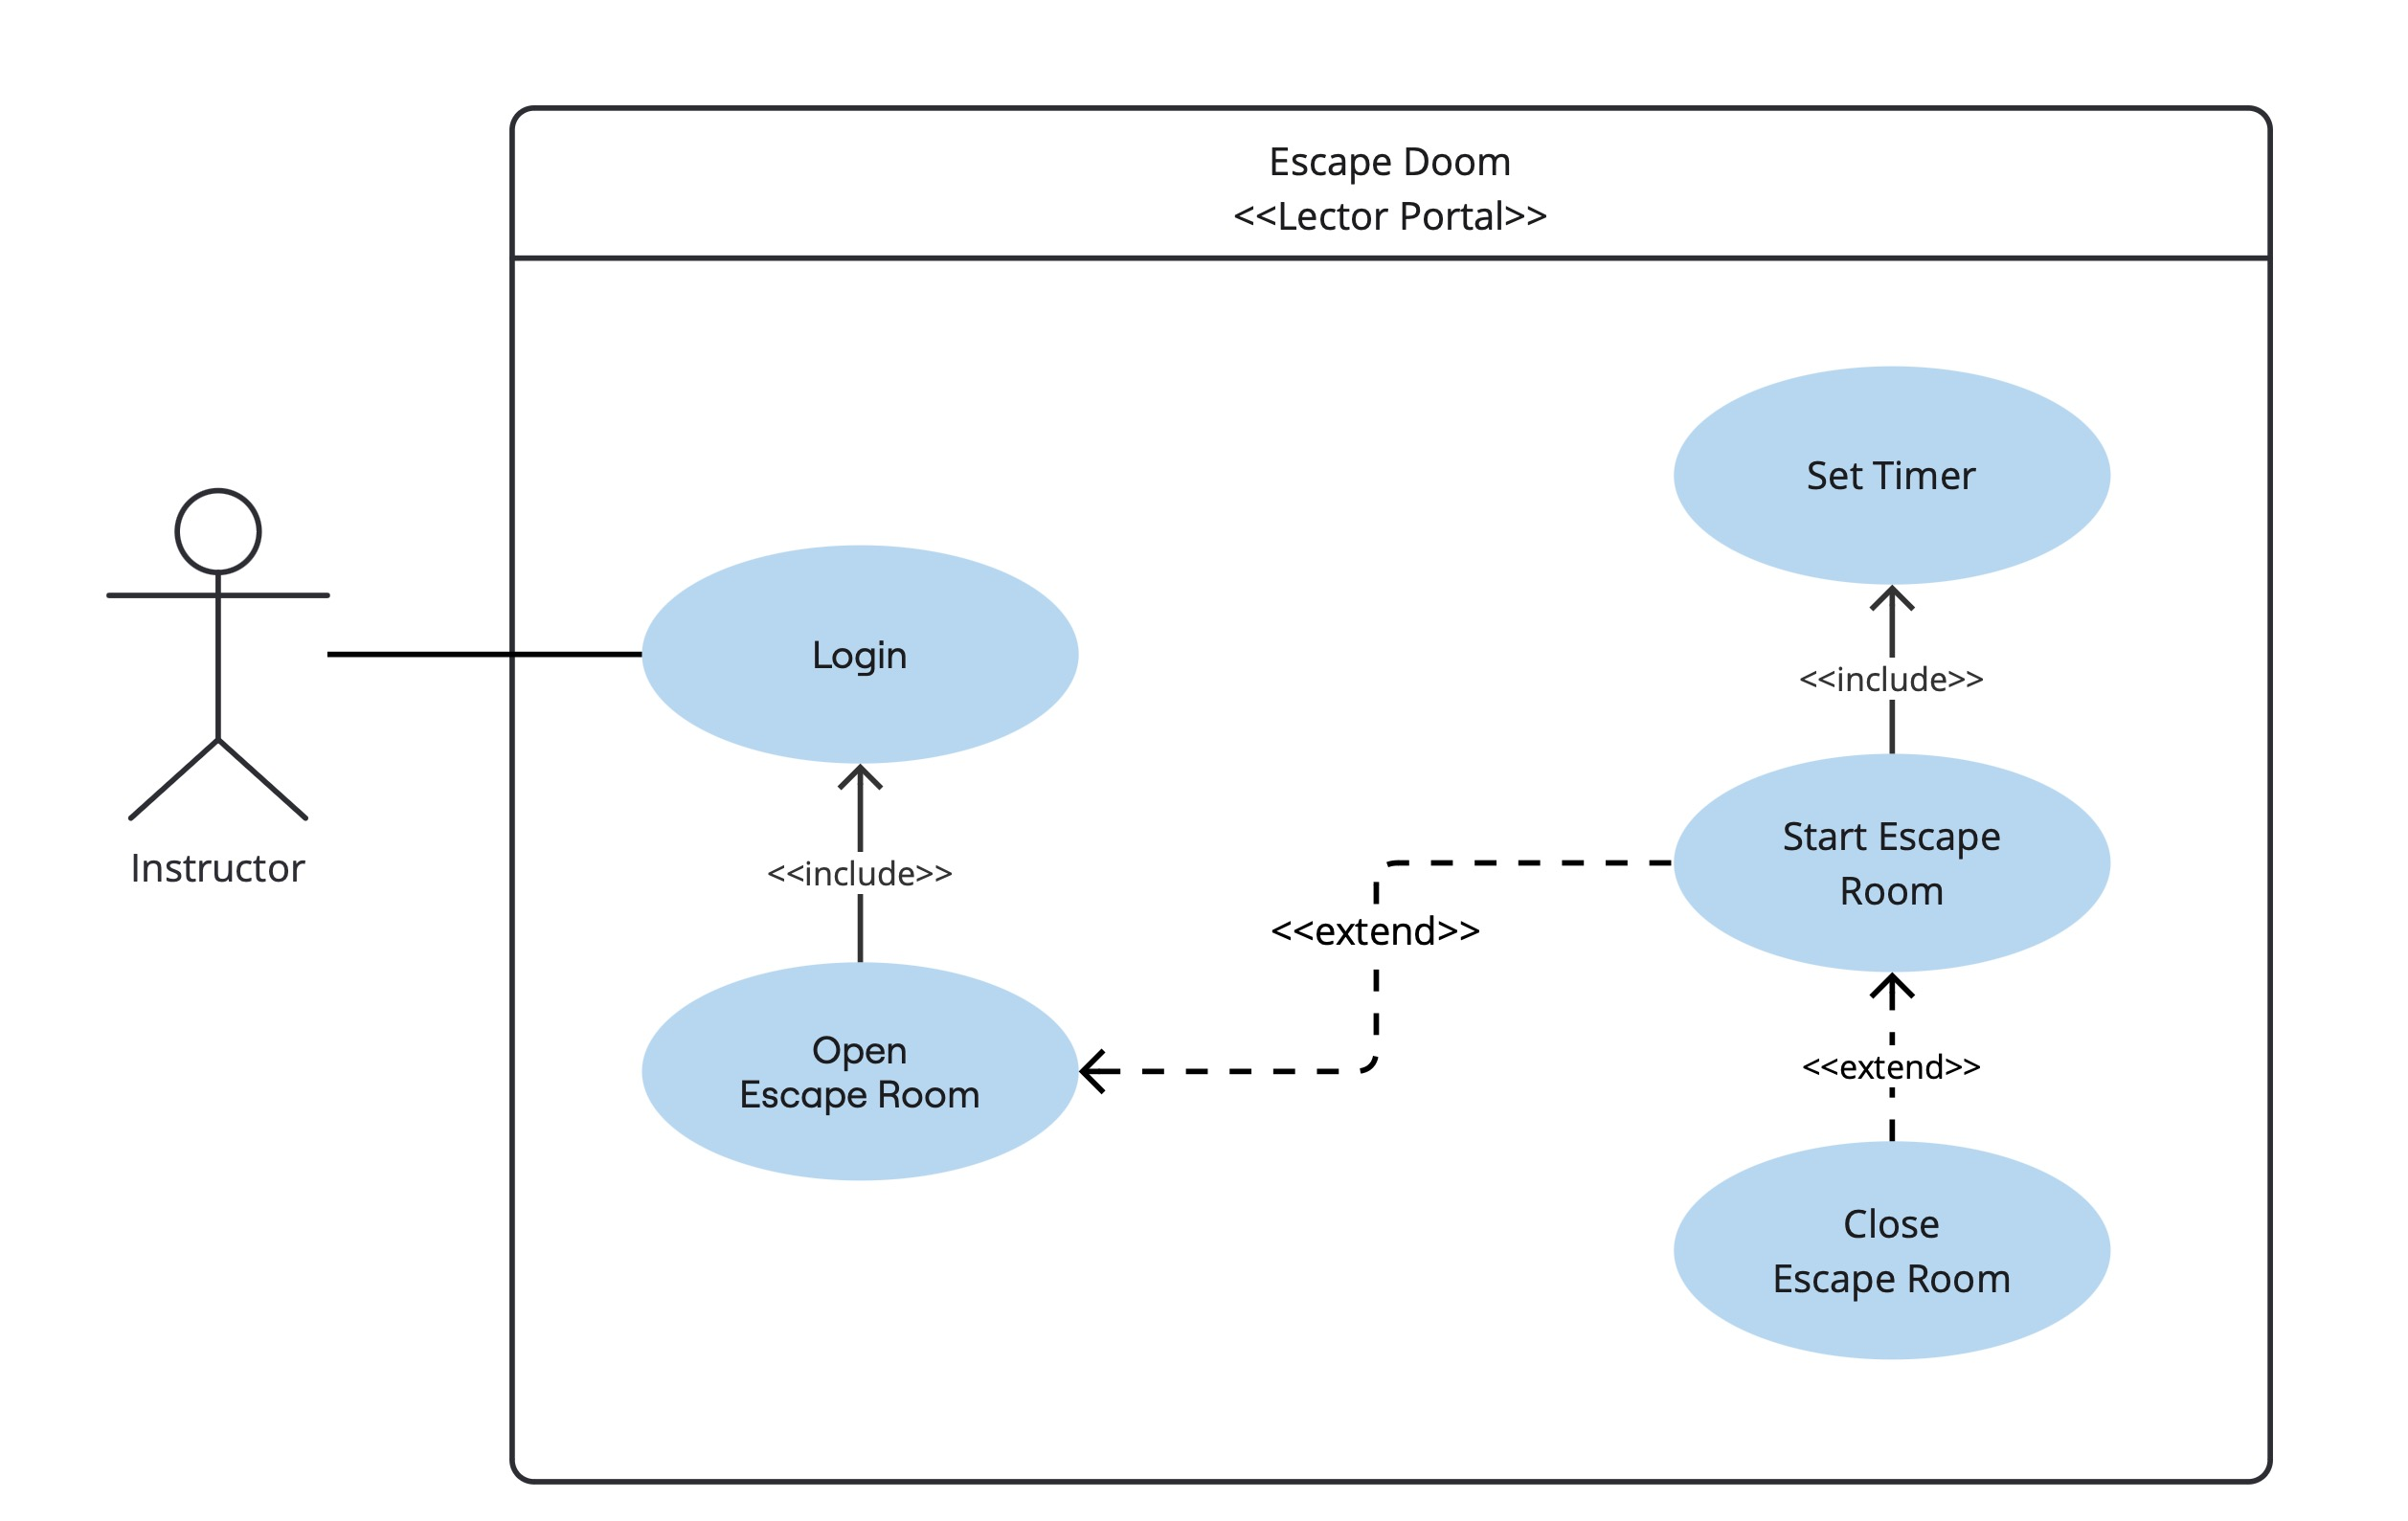
\includegraphics[width=\linewidth]{UC-01.png}
    \caption{UC01 - Lector Portal}
    \label{fig:uc-01}
\end{figure}



\begin{figure}[h!]
    \centering
    \includegraphics[width=\linewidth]{images/LectorPortal.png}
    \caption{Lector Portal Mockup}
    \label{fig:lector:portal}
\end{figure}


\begin{figure}[h!]
    \centering
    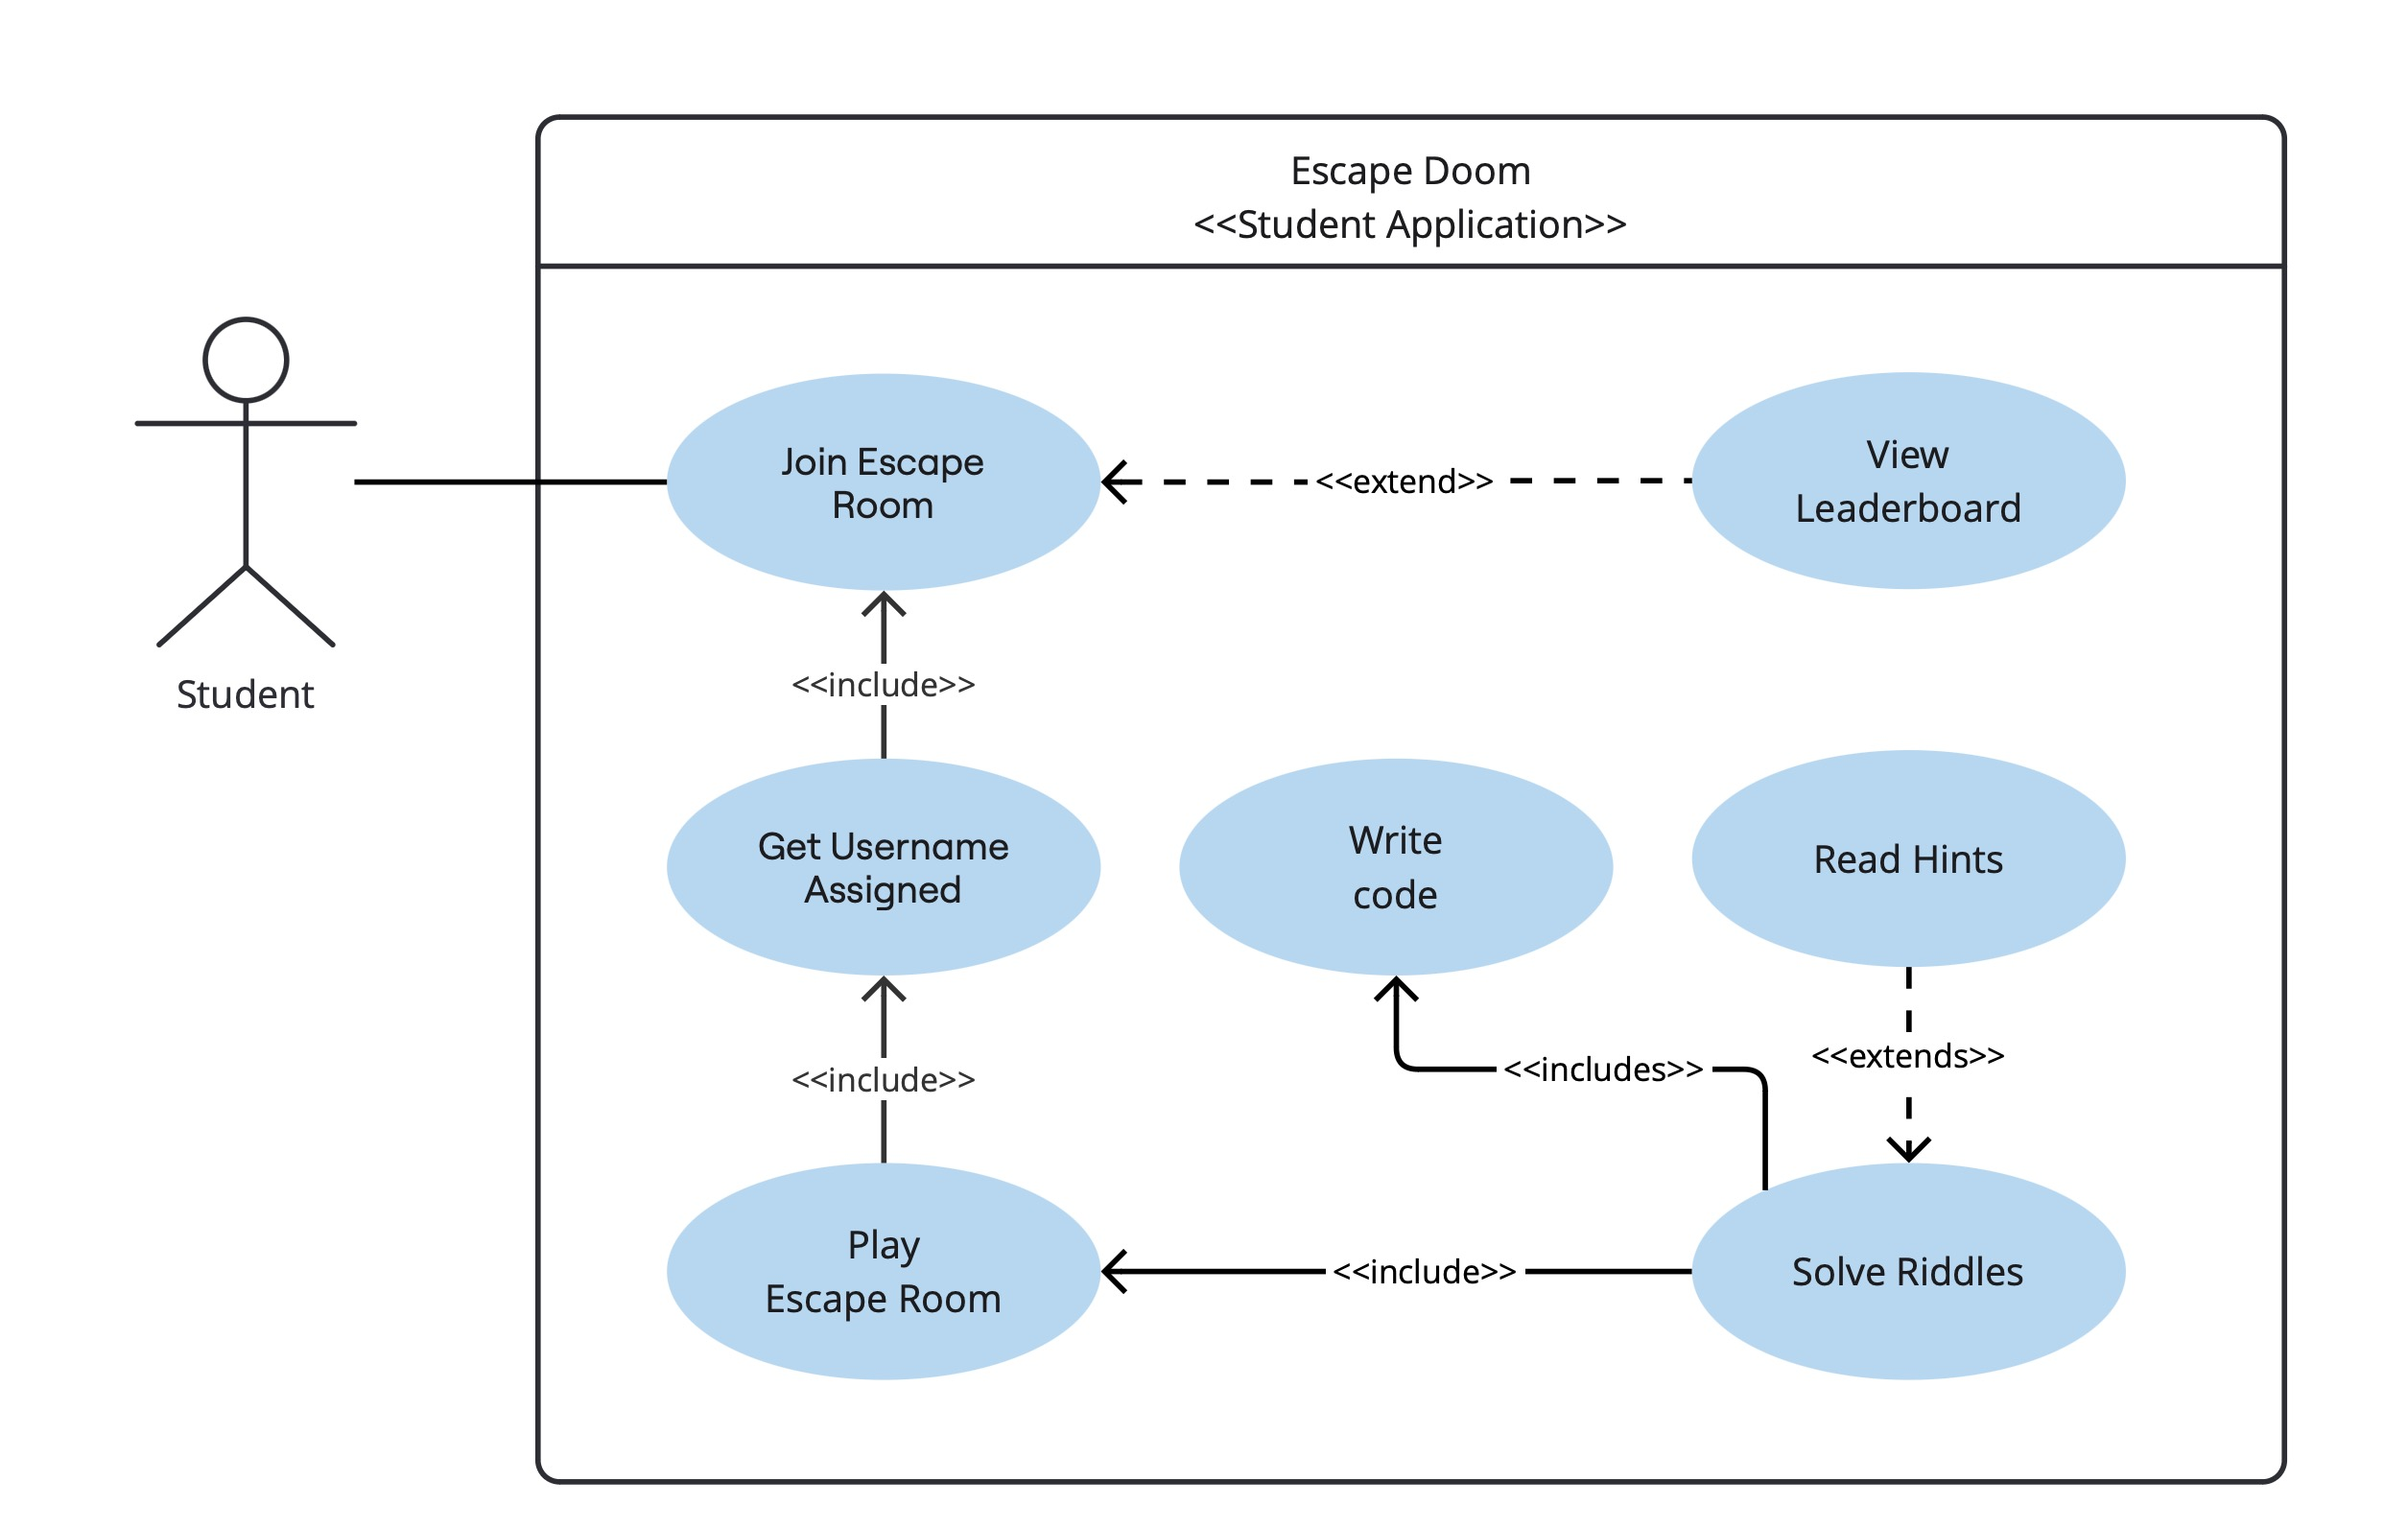
\includegraphics[width=\linewidth]{UC-02.png}
    \caption{UC02 - Student Application}
    \label{fig:uc-02}
\end{figure}
\newpage

\begin{figure}[h!]
    \centering
    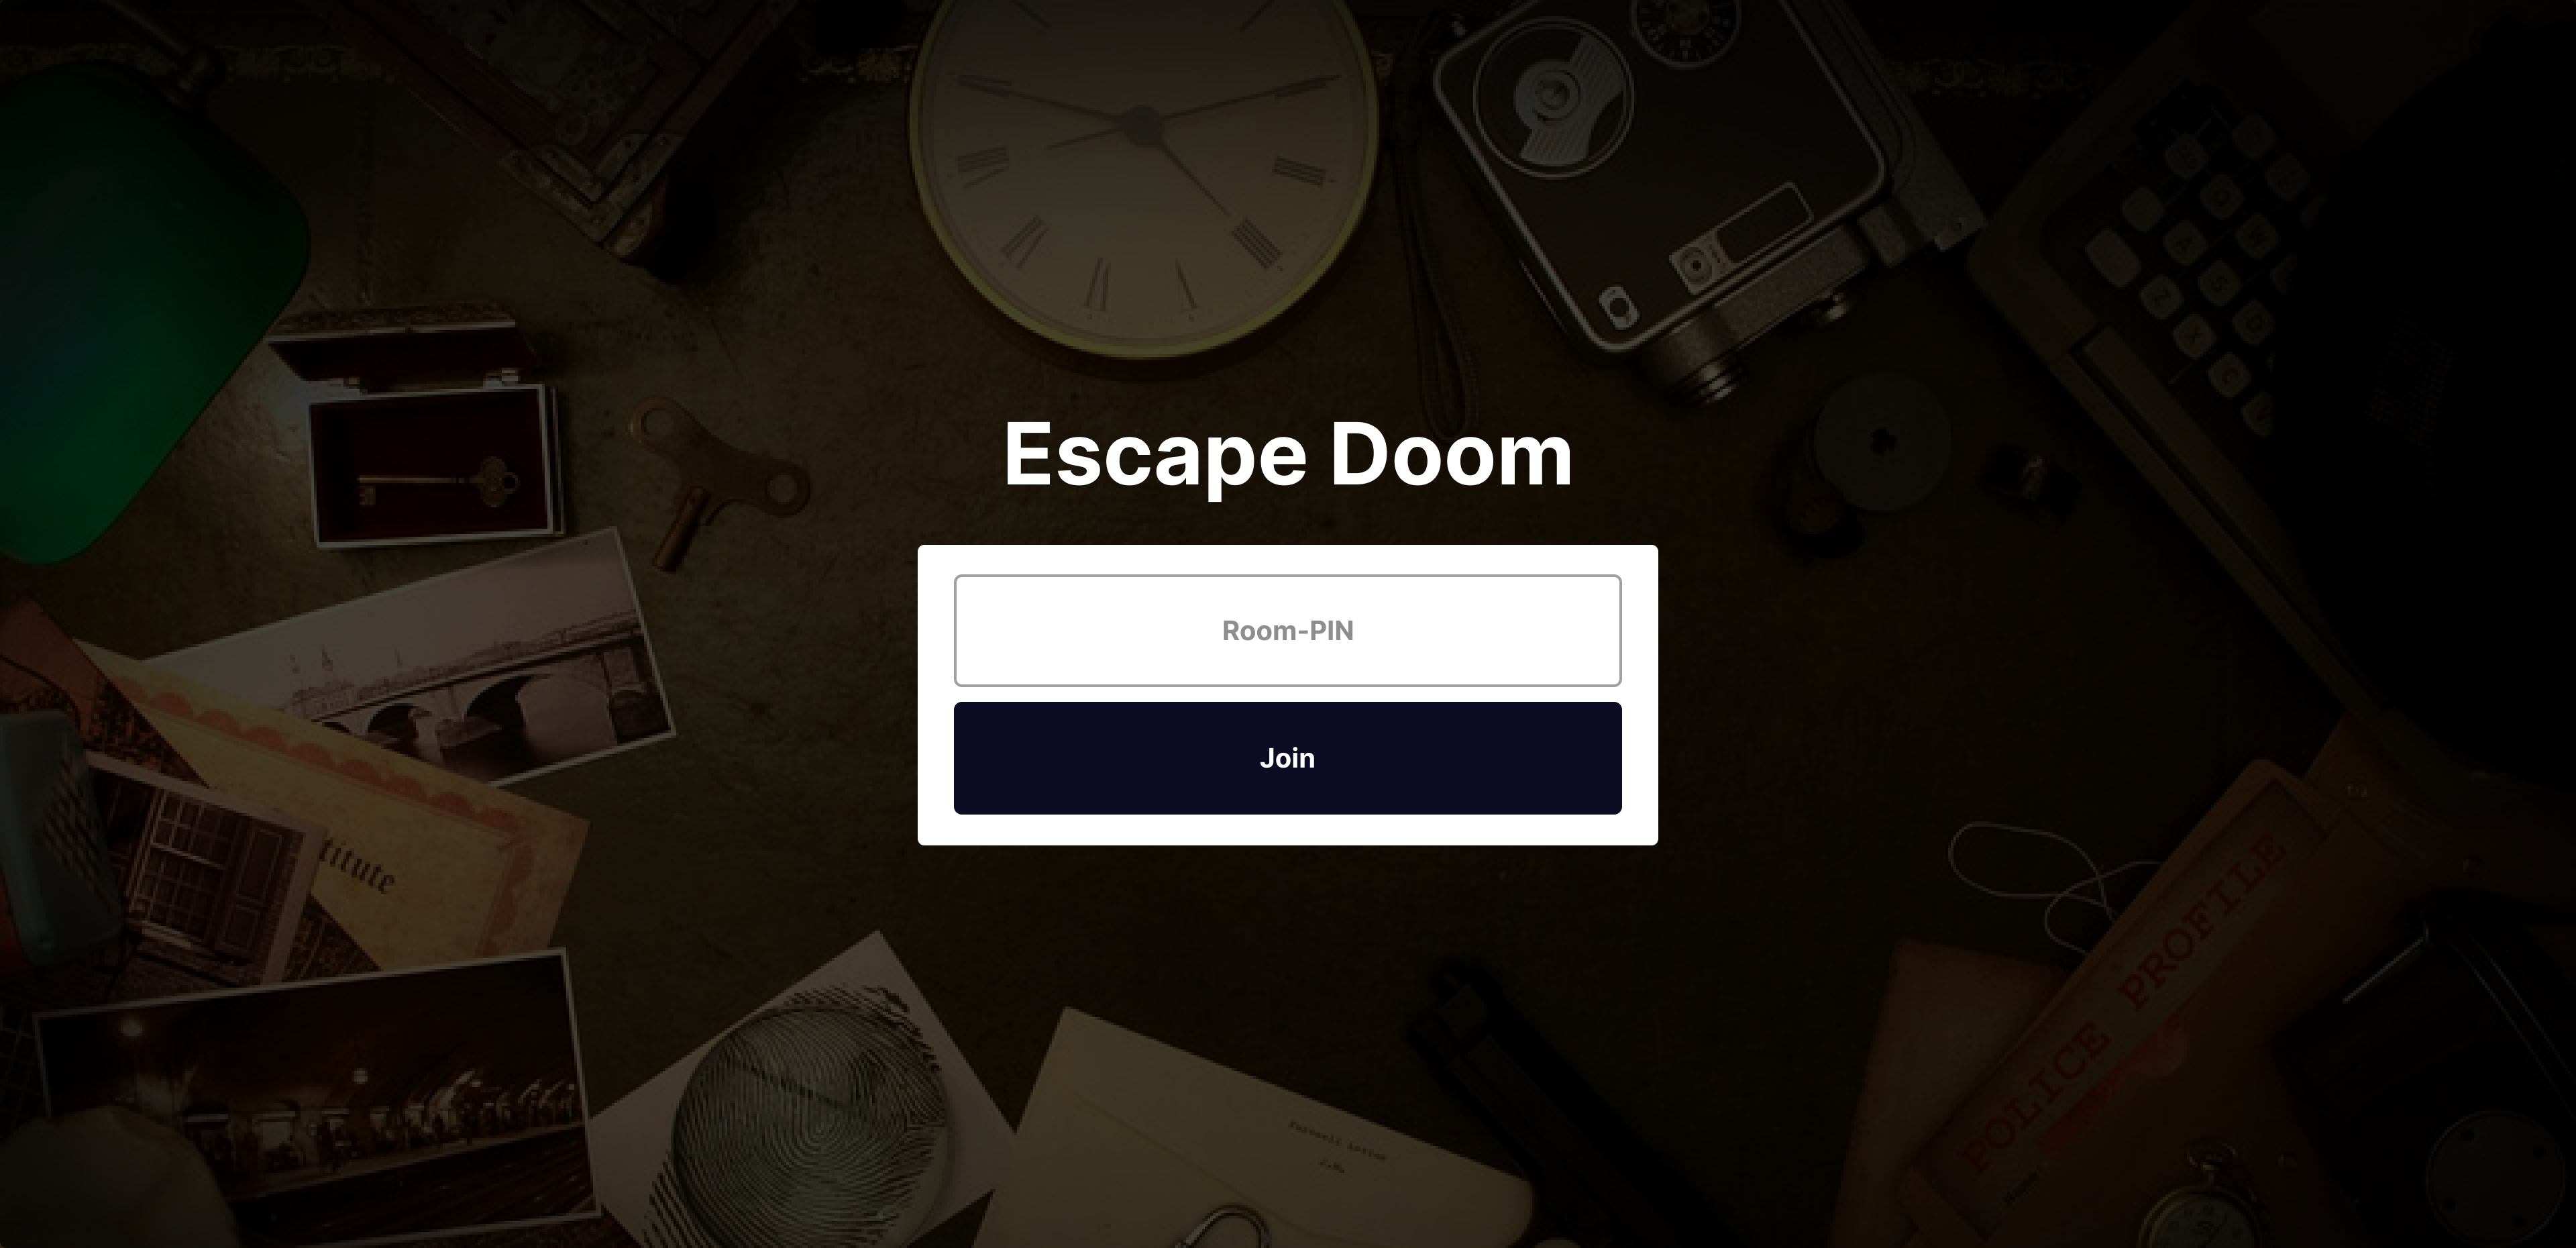
\includegraphics[width=\linewidth]{images/StudentJoin.png}
    \caption{Student Application Mockup}
    \label{fig:lector:portal}
\end{figure}
\section{Relevant Product Risks}\label{sec:relevant-product-risks}

This chapter identifies the primary product-level risks associated with the Escape Doom system, based on its context, architectural strategy, and intended use. These risks are relevant to ensuring the platform delivers a reliable and maintainable experience for both students and lecturers of FH Campus Wien.

\subsection*{Context-Based Risk Identification}

The Escape Doom system enables lecturers to manage escape rooms and students to participate in them through a shared browser-based interface. Key software and systems involved include:

\begin{itemize}
    \item \textbf{Frontend (Next.js):} Unified interface for students and lectors.
    \item \textbf{Backend (Spring Boot Microservices):} Business logic separated by domain (e.g., game management, user sessions).
    \item \textbf{Code Executor Service:} Executes user-submitted code (externalized via API).
    \item \textbf{Image Hosting Service:} Provides visual assets used in room puzzles.
    \item \textbf{Authentication Provider:} Handles identity and access control.
\end{itemize}

These components interact across runtime boundaries, which introduces integration and reliability challenges that must be mitigated by effective testing.

\subsection*{Risks Derived from the Solution Strategy}

\begin{tabularx}{\textwidth}{|p{5cm}|X|}
    \hline
    \textbf{Risk Category} & \textbf{Description} \\
    \hline
    Deployment Configuration Errors &
    Kubernetes-based deployment introduces risk in service discovery, routing, and persistence, especially when deploying updates to stateless services. \\
    \hline
    Data Loss or Corruption &
    Mismanagement of externalized state (e.g., Redis, PostgreSQL) may lead to lost game progress or broken leaderboard data. \\
    \hline
    Security Misconfigurations &
    Improper gateway configuration or missing authentication checks could expose APIs or user data, especially since third-party services like Code Executor are integrated. \\
    \hline
    Frontend Failure or Desync &
    Since a single Next.js application serves both user groups, any frontend bug can affect all flows. Moreover, inconsistency between client state and backend responses may lead to corrupted game flows. \\
    \hline
    Performance Degradation Under Load &
    Scalability is a stated goal, but it comes with the risk that system components (especially custom services) may not scale equally, leading to degraded UX. \\
    \hline
    Code Execution Instability &
    As the Code Executor is an externalized subsystem, failures or incorrect behavior in this service can block entire escape room flows. \\
    \hline
    Inter-Service Communication Failures &
    The system relies heavily on service-to-service calls (e.g., Spring Cloud Gateway). Misrouting, timeouts, or schema mismatches can disrupt game logic. \\
    \hline
\end{tabularx}

\subsection*{Test-Relevant Risk Dimensions}

Each risk will be further analyzed along three key dimensions during test design:

\begin{itemize}
    \item \textbf{Likelihood:} How likely is this risk to occur given current implementation and system context?
    \item \textbf{Impact:} What would be the consequence to user experience or data integrity if the risk occurred?
    \item \textbf{Detectability:} Can this issue be easily discovered during development or testing?
\end{itemize}

These will help prioritize test effort and define test depth and scope for each risk area.

\subsection*{Implications for System Quality}

The product risks identified above point to areas where the system’s quality could be compromised if not properly addressed during testing. Several architectural decisions such as splitting the backend into microservices, using external services for code execution, and relying on runtime communication—introduce specific challenges that could affect both user experience and system robustness.

For example, inter-service dependencies may lead to cascading failures, which makes resilience and fault tolerance essential. The integration of external components, like the Code Executor, creates additional attack surfaces and reliability concerns that must be mitigated through isolation and fallback mechanisms.

Ensuring smooth frontend-backend interaction is key to maintaining a consistent game flow, while performance bottlenecks during peak usage could directly impact the responsiveness expected by students and instructors.

These risks underline the importance of focusing testing efforts on aspects such as maintainability, availability, data integrity, security, and overall system responsiveness. Addressing these proactively in the test design will support the delivery of a stable, usable, and secure application.

Testing will therefore be closely aligned with these quality characteristics to reduce the likelihood and impact of such risks.

\section{Quality Requirements}
\label{section-quality-requirements}

\subsection*{Quality Overview Table}

\begin{longtable}{|p{4.2cm}|p{6.8cm}|p{5.8cm}|}
    \hline
    \textbf{Category} & \textbf{Requirement / Sub-Goal} & \textbf{Scenario} \\
    \hline
    \textbf{Functionality} &
    \begin{itemize}
        \item Instructor login and room management
        \item Student interaction with rooms
        \item Code editor syntax highlighting
        \item Real-time leaderboard updates
    \end{itemize} &
    \begin{itemize}
        \item Scenario 1: Instructors log in securely to manage rooms
        \item Scenario 2: Leaderboards update after solving riddles
    \end{itemize} \\
    \hline
    \textbf{Performance} &
    \begin{itemize}
        \item Handle 200 concurrent users
        \item Code execution within 10 seconds
    \end{itemize} &
    \begin{itemize}
        \item Scenario 1: High concurrency in a single room
        \item Scenario 2: Fast result feedback for code
    \end{itemize} \\
    \hline
    \textbf{Usability} &
    \begin{itemize}
        \item Join room in under one minute
        \item Visible hints on all screen sizes
    \end{itemize} &
    \begin{itemize}
        \item Scenario 1: Fast room joining
        \item Scenario 2: Hints visible on various devices
        \item Scenario 3: Keyboard navigation for all actions
    \end{itemize} \\
    \hline
    \textbf{Reliability} &
    \begin{itemize}
        \item Persistent progress after browser cache is cleared
        \item Handle malicious code without crashing
        \item Keep core features during partial outage
    \end{itemize} &
    \begin{itemize}
        \item Scenario 1: Progress restoration after cache clear
        \item Scenario 2: System stability on bad input
        \item Scenario 3: Maintain basic features during failure
    \end{itemize} \\
    \hline
    \textbf{Security} &
    \begin{itemize}
        \item Prevent unauthorized access
        \item Sandbox for code execution
        \item Encrypted communication
    \end{itemize} &
    \begin{itemize}
        \item Scenario 1: Block access on login failure
        \item Scenario 2: Run code in isolation
        \item Scenario 3: Use HTTPS for all communication
    \end{itemize} \\
    \hline
    \textbf{Data Integrity} &
    \begin{itemize}
        \item Secure storage of results
        \item Backup and recovery
    \end{itemize} &
    \begin{itemize}
        \item Scenario 1: Restore leaderboard after crash
        \item Scenario 2: Recover from backup in 10 minutes
    \end{itemize} \\
    \hline
    \textbf{Accessibility} &
    \begin{itemize}
        \item WCAG 2.1 compliance
        \item Support for color blindness
    \end{itemize} &
    \begin{itemize}
        \item ---
    \end{itemize} \\
    \hline
\end{longtable}

\section{Derived Test Objectives}
\label{section-derived-test-objectives}

Based on the identified product risks and defined quality requirements, the following test objectives have been established to guide test design and prioritization:

\begin{itemize}
    \item \textbf{Verify system stability across microservices}, ensuring failures in one service do not propagate and that fallback or error handling is in place.

    \item \textbf{Test secure user authentication and role management}, validating that only authorized users can access protected features and user data is handled securely.

    \item \textbf{Validate persistent and correct game state management}, including user progress, session data, and leaderboard synchronization, even in failure scenarios.

    \item \textbf{Confirm code execution behavior is safe and reliable}, particularly in handling edge cases, incorrect input, or malicious submissions.

    \item \textbf{Assess frontend usability and responsiveness}, especially in terms of navigation, accessibility, and performance across devices and screen sizes.

    \item \textbf{Check system performance under expected concurrency}, ensuring smooth operation with up to 200 users per room and acceptable response times.

    \item \textbf{Ensure recoverability and data integrity}, with proper test coverage for backup, restore, and resilience mechanisms in the case of data loss or outages.

    \item \textbf{Verify CRUD operations in all repositories}, ensuring that each microservice managing a domain entity has complete test coverage for Create, Read, Update, and Delete functionality. This applies to all persistent components within the system.
\end{itemize}

These objectives reflect the test priorities and help define the focus areas for unit and system-level testing. Each objective will be mapped to specific test cases in later test design phases.

\section{Unit Test Approach}
\label{section-unit-test-approach}

\subsection*{General Approach}

Unit tests are written following a Test-Driven Development (TDD) strategy where applicable, particularly during the early stages of service implementation. Tests are focused on public methods. Private methods are not tested directly, as their logic is implicitly validated through the public interface.

Each microservice follows a consistent folder structure to support maintainable and repeatable testing workflows. When upper layers (e.g., services or controllers) are introduced, previously granular tests may be reduced to improve build speed while still ensuring coverage through layered validation.

\subsection*{Test Structure by Domain Service}

\paragraph{Data Service}
As a core service, the data service maintains the highest test coverage:

\begin{itemize}
    \item \textbf{Data access layer:} 62\% of classes, 74\% of lines covered
    \item \textbf{Mapping layer:} 90\% of classes, 53\% of lines covered
    \item \textbf{Service layer:} 100\% of classes, 83\% of lines covered
\end{itemize}

Testing began with TDD to ensure all repositories implement and verify CRUD operations. Service-layer tests validate integration with data handlers and repositories. Flyway is also integrated to provide a stable schema for testing.

\paragraph{Leaderboard Service}
This service is not yet fully implemented. Testing is planned as follows:

\begin{itemize}
    \item \textbf{Unit tests} will focus on transformation logic between session data and leaderboard models.
    \item \textbf{Edge cases} such as empty result sets and invalid session responses will be covered.
    \item \textbf{Risk-based focus:} Inaccurate or missing leaderboard data could break user trust, so correctness and reliability are critical.
\end{itemize}

\paragraph{Player Service}
Current coverage status:

\begin{itemize}
    \item \textbf{Data access layer:} 33\% of classes, 18\% of lines
    \item \textbf{Service layer:} 84\% of classes, 18\% of lines
\end{itemize}

Further testing is required to reach at least 60\% line coverage. Focus areas include data integrity, score calculation logic, and boundary conditions for user progress tracking.

\paragraph{Session Service}
Already has strong test coverage:

\begin{itemize}
    \item \textbf{Data access layer:} 100\% of classes, 80\% of lines
    \item \textbf{Service layer:} 100\% of classes, 36\% of lines
\end{itemize}

Remaining work includes covering more complex logic branches in the service layer, particularly scenarios with invalid session states or timing constraints.

\paragraph{Gateway Service}
As this component mainly handles routing and security, its logic will be validated through frontend end-to-end and system integration tests rather than unit tests.

\subsection*{Test Tools}
\begin{itemize}
    \item \texttt{JUnit 5} for all Java service-level tests
    \item \texttt{Mockito} for mocking dependencies in isolation
    \item \texttt{Flyway} for consistent schema migration and rollback in test environments
\end{itemize}

\section{System Test Approach}
\label{section-system-test-approach}

System testing plays a critical role in validating that all components of the Escape Doom platform work together as expected from an end-user perspective. While unit and integration tests focus on isolated components and internal logic, system tests verify real-world behavior across services, interfaces, and layers.

\subsection*{Test Basis}
System tests are based on:
\begin{itemize}
    \item Functional specifications
    \item Use cases for both student and lecturer roles
    \item Previously identified product risks and quality goals
\end{itemize}

\subsection*{Test Objects}
\begin{itemize}
    \item Complete microservice-based application stack (frontend, backend, gateway)
    \item End-to-end flows such as:
    \begin{itemize}
        \item Joining and playing an escape room
        \item Submitting and evaluating code
        \item Viewing and updating the leaderboard
        \item Session management by instructors
    \end{itemize}
\end{itemize}

\subsection*{System Testing Strategy}

The system tests are primarily conducted through **end-to-end (E2E) automation**, simulating realistic user behavior across the application stack. These tests aim to ensure that key user-facing functionality remains intact during development cycles.

\begin{itemize}
    \item \textbf{E2E Tests with Playwright and Selenium:} Used to simulate browser-based interaction scenarios involving students and lecturers. This ensures that critical user workflows (e.g., login, code submission, viewing leaderboards) work across services and through the UI.

    \item \textbf{MockMVC Tests:} Used within backend services to simulate HTTP requests at the controller level. This allows us to test edge cases, error handling, and validation logic without requiring a full UI-driven scenario.
\end{itemize}

\subsection*{Test Tools}
The team has agreed on the following tools to support system and controller-level testing:

\begin{itemize}
    \item \textbf{Playwright / Selenium} – For simulating real user actions and full-stack testing.
    \item \textbf{MockMVC} – For controller tests, especially useful where UI coverage is not sufficient.
    \item \textbf{TestContainers} – To create realistic, isolated test environments with actual database instances.
    \item \textbf{AssertJ} – For fluent and human-readable assertions in all Java-based tests.
\end{itemize}

\subsection*{Why System Tests Are Important}

Given our microservice architecture and external dependencies (e.g., Code Executor, Authentication Provider), integration and contract errors may not be caught at the unit level. System tests help verify:

\begin{itemize}
    \item Cross-service communication and data flow
    \item User-visible behavior consistency
    \item Fault tolerance and error handling under real conditions
    \item Confidence in critical flows such as progress tracking and leaderboard updates
\end{itemize}

\include{chapters/7. Test_Infrastructure}

\end{document}
